\chapter{Datenbank \& 2D vs 3D Unterschied}
\label{\docname}
In diesem Kapitel wird die Umsetzung von der Datenbank sowie auch die Differenzierung zwischen 3D und 2D Gesichtern besprochen. Es wird zuerst eine allgemeine Beschreibung gemacht, danach werden allen Schritten von der Plan Phase bis zu der Implementierungsphase besprochen. Allen Problemen, Herausforderung und Ergebnissen dieses Teil des Projektes werden genau erklärt.
\section{Umsetzung}
In der folgenden Tabelle werden alle Technologien, die mit diesem Teilbereich des Projekts  zu tun haben. Zuerst wird eine allgemeine Erklärung der Technologie gemacht, und danach werden mehr Details beschrieben, wie z.B die verwendeten Bibliotheken bzw. wieso diese gewählt wurden. Diese Beschreibung ist für sowie die Datenbank und den 2D vs. 3D Unterschied.

\begin{table}[ht]
	\centering
	\begin{tabular}{ |l|l|l| } 
		\hline		
		Technologie & Beschreibung & Lizenz \\ 
		\hline
		MySQL & Datenbankverwaltungssystem & Kostenlos \\ 
		\hline
		MariaDB & Datenbankverwaltungssystem & Kostenlos \\
		\hline 
		Python & Objekte-orientierte Programmiersprache & Kostenlos \\
		\hline 
		OpenCV &  Bildverarbeitung Programmbibliothek  & Kostenlos \\ 
		\hline
	\end{tabular}
	\caption{Technologien}
	\label{table:tech}
\end{table}
\subsubsection{MySQL}
\begin{figure}
	\centering
	\includegraphics[scale=0.3]{\ordnerfigures mysql.jpg}
	\caption{ MySQL Logo}
	\label{fig:mysql}
	\cite{MySQLlogo}
\end{figure}
\textit{"MySQL ist eine CLient/Server
Implentierung, die aus einem Server-Dämon mysqld und vielen Client Programmen, sowie
Bibliotheken für PERL, PHP/3, PHP/4 sowie ASP besteht.
SQL ist eine standardisierte Datenbanksprache, die das Speichern, Updaten und den Zugriff auf
Informationen erleichtert. Beispielsweise kann man Produktinformationen eines Kunden auf einem
WWW-Server speichern und abrufen. MySQL ist äußerst schnell und flexibel genug, um sogar Bilder
und Log-Dateien darin abzulegen. In der Praxis ist MySQL sehr viel schneller, als z.B. ORACLE oder INFORMIX."}\cite{stepken1999mysql}
\bigbreak
MySQL hat ein breites Anwendungsspektrum und wird meistens in Verbindung mit PHP, Linux, Python usw. verwendet. Der Grund warum MySQL verwendet wird, ist die einfache Bedienung und Verwaltung dieser Datenbank. Da es sich bei diesem DBS um eines der am häufigsten verwendeten DBS handelt, gibt es eine Vielzahl von Tools, die zum Verwalten der Datenbank verwendet werden können.

\subsubsection{MariaDB}
\textit{"MariaDB ist aktuell die am schnellsten wachsende Open-Source-Datenbanklösung. Sie wird hauptsächlich von der MariaDB Corporation entwickelt und ist ein Fork von MySQL. Mittlerweile bietet das Datenbankverwaltungssystem mit seinen diversen kostenfreien Features vieles, was MySQL nicht oder nur kostenpflichtig zur Verfügung stellt (z.B. eine Speicher-Engine zur performanten Verarbeitung von riesigen Datenmengen; ein Datenbank-Proxy zur sicheren und hoch-verfügbaren Verwaltung skalierbarer Installationen u.v.m.). Im Gegensatz zu MySQL verfügt MariaDB jedoch nicht über einen eigenen Client wie die Workbench. Eine gute kostenfreie Alternative stellt HeidiSQL dar, jedoch verfügt diese über kein Dashboard, welches z.B. die Funktionsweise des Servers darstellt und damit Optimierungsentscheidungen erleichtert."}\cite{MariaDB-Monitor}
\begin{figure}[h]
	\centering
	\includegraphics[scale=0.3]{\ordnerfigures mariadb.png}
	\caption{ MariaDB Logo}
	\label{fig:mariadb}
	\cite{MariaDBlogo}
\end{figure}
\bigbreak
Es ist hauptsächlich für Linux ausgelegt. Es bietet eine einfache Verbindung mit Linux-Betriebssystem so wie auch mit Python, C ++ und vielen anderen Programmiersprachen. Da dies der Standard-Linux-DBS ist und unsere Software unter Linux mit Python-Skripten geschrieben wurde, ist MariaDB das DBS unserer Wahl.

\subsubsection{Python}
Python ist eine Programmiersprache, die der User mit seiner einfachen Syntax hilft. Für die meisten Betriebssysteme ist Python frei zur Verfügung gestellt. Alles was mit Objektorientierung zu tan hat, wird im Python unterstützt und weiterentwickelt.\\
\cite{pythonInfo}
\begin{figure}[ht]
	\centering
	\includegraphics[scale=0.3]{\ordnerfigures python.png}
	\caption{ Python Logo}
	\label{fig:python}
	\cite{Pythonlogo}
\end{figure}
 Die Sprache weist ein offenes, gemeinschaftsbasiertes Entwicklungsmodell auf, das durch die gemeinnützige Python Software Foundation gestützt wird, die de facto die Definition der Sprache in der Referenzumsetzung CPython pflegt.

\bigbreak
Der Grund, warum die Software in Python geschrieben wurde, legt an der einfachen und schnellen Möglichkeit, um Datenbankskripte und Gesichtserkennungsprogramme zu erstellen.
\subsubsection{OpenCV}
OpenCV (Open Source Computer Vision Library) ist eine Open-Source-Bibliothek für Machine Learning Programme und Computer Vision Software. Der Grund zur Entwicklung von OpenCV ist, eine Moglichkeit anzubieten, wo Objekte analysiert und erkennt bzw. identifiziert werden. Der Code von OpenCv ist leicht nutzbar und änderbar, weil es als BSD Produkt lizenziert ist. Es ist von Windows, Linux, Android und Mac verfügbar und unterstützt.\cite{OpenCV1}
\begin{figure}[ht]
	\centering
	\includegraphics[scale=0.3]{\ordnerfigures opencv.png}
	\caption{ OpenCV Logo}
	\label{fig:opencv}
	\cite{OpenCVlogo}
\end{figure}
\bigbreak
Obwohl es in C ++ geschrieben wurde, bietet es viele Schnittstellen zu anderen Programmiersprachen wie Python, die in diesem Projekt implementiert werden. OpenCV ist eine plattformübergreifende Bibliothek und da es viele Deep-Learning-Algorithmen und Frameworks enthält, ist unsere Wahl für die Objekterkennung.

\section{Technische Lösungen}
In diesem Teilbereich werden die Technischen Lösungen bzw. die Planung und Implementierung der verschiedenen Aufgaben der Datenbank und Gesicht-Spoofing Erkennung erklärt.
\subsection{Datenkbank}
Wie bereits erwähnt, haben wir uns für MySQL und MariaDB als DBS entschieden, wobei meistens das zweite zum Einsatz kommt. Es ist wichtig zu beachten, dass die Datenbank nicht über die Befehlszeile oder die MySQL/MariaDB-Konsole angesprochen wird, sondern mithilfe von Python-Skripten. In diesem Fall würde jeder gegebene Befehl in den Python-Dateien gespeichert, und wenn etwas schief ging, konnten die Skripte einfach verbessert und Fehler behoben werden.
\bigbreak
Um eine Datenbank zur Gesichtserkennung und -identifikation zu entwerfen, mussten einige Nachforschungen angestellt werden, bei denen es hauptsächlich darum ging, Beispiele für vorhandene Datenbanken zu finden. Auf diese Weise konnten wir uns eine Vorstellung davon machen, wie Datenbanken aussehen. Obwohl die meisten Datenbanken nicht kostenlos waren und einige Unterlagen unterschrieben werden mussten, um die vollständigen Details zu erhalten, war dies mehr als ausreichend, um einen Ausgangspunkt zu haben. Einige der gefundenen Datenbanken sind:
\begin{itemize}
	\item 3D Mask Attack Dataset\cite{Database1}
	\item The AR Face Database, The Ohio State University\cite{Database2}
	\item Caltech Faces\cite{Database3}
	\item CAS-PEAL Face Database\cite{Database4}
	\item The Color FERET Database, USA\cite{Database5}
\end{itemize}
Auf den ersten Blick scheint es nicht sehr schwierig zu sein, eine Gesichtserkennungsdatenbank zu erstellen, aber da sich das Projekt entwickelte, mussten viele Änderungen vorgenommen werden, da sie an die Gesichtsdaten der Person weitergegeben wurden.
\bigbreak
Der nächste Schritt bestand darin nachzuforschen, wie in Python die Schnittstelle mit MariaDB aussehen. Davon vielen Linux-Benutzern empfohlen wurde, Python für die Verbindung zu MariaDB zu wählen, wurde der Programmierer aufgefordert, den Code mithilfe von Methoden und try and except-Anweisungen zu schreiben, um saubere Skripte zu erstellen. Auf diese Weise würde der Code sehr einfach zu analysieren und zu verbessern sein, damit die Fehlermeldungen je schnell wie möglich zu beseitigen.
\subsubsection{Beschreibung der Tabellen}
Nach der Anfangsplanung wurden die folgenden zwei Tabellen definiert:
\begin{itemize}
	\item Person
	\item Log
\end{itemize}
\begin{figure}[!htb]
  \centering
    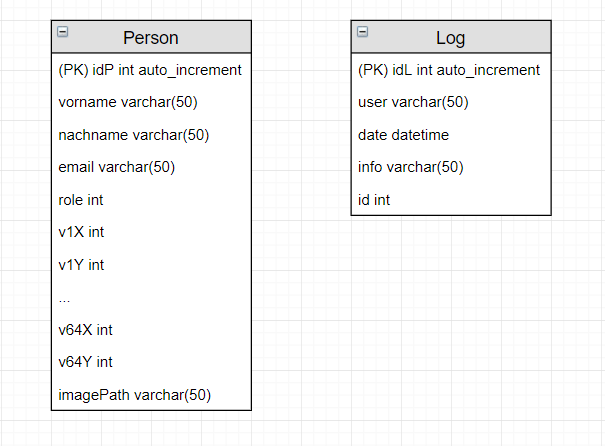
\includegraphics[width=0.8\textwidth]{./figures/db.png}
      \caption{Datenbank - RDM}
\end{figure}
\subsubsection{Tabelle Person}
Die erste Tabelle, Person, enthält alle User mit ihren grundlegenden Informationen, wie Vorname, Nachname, Rolle, Email, Gesichtspunkten sowie auch der Pfad von dem Bild. Die Benutzer des Systems werden in zwei Gruppen, Admin und normaler User, geteilt. Damit es einen Unterschied zwischen diesen beiden Gruppen gibt, gibt es die Spalte Rolle. Diese Spalte bekommt als Wert die Zahl 1, wenn der Person ein Admin ist, und die Zahl 0 für einen normalen Users.
\bigbreak
Die Spalte idP ist eine eindeutige Spalte, die es für dieIdentifizierung als die Datenzeile gibt, deshalb wird sie als Primar Schlüssel definiert. Sie wird auch auto increment definiert, damit die Tupel automatisch nummeriert werden.
\bigbreak
Die Spalte Nachname enthält den Nachname der Person, deshalb wird sie als Datentyp Varchar mit der Lange 50 gespeichert, weil Varchar zum Speichern von Strings geeignet ist.
\bigbreak
Die Spalte Email enthält die Email der Person, deshalb wird als Datentyp Varchar mit der Lange 50 gespeichert, weil Varchar zum Speichern von Strings geeignet ist.
\bigbreak
Die Spalte Rolle enthält die Rolle der Person, deshalb wird als Datentyp Char mit der Lange 1 gespeichert, weil Char zum Speichern von Strings geeignet ist. Um eine einfache Nummer zu speichern, ist hier auch den Datentyp Int verwendbar.
\bigbreak
Jeder Punkt besteht aus eine X und Y Koordinate, und von jedem Bild gibt es einen Startpunkt, wo die anderen Punkten relativ zu diesem Punkt gespeichert werden. Für diese Punkte wird den Datentyp decimal werden, weil die Koordinaten Kommazahlen sind. Insgesamt werden von einem Bild 64 Gesichtspunkten gespeichert.
\bigbreak
Die Spalte imagePath speichert den Pfad der Bilder und wird mit dem Datentyp Varchar mit einer Länge von 50 gespeichert, weil Varchar zum Speichern von Strings geeignet ist. Die Bilder werden mit ihrem Pfad und nicht als ganze Bilder gespeichert, weil wenn diese Bilder in der Datenbank gespeichert werden, würde die Datenbank überfüllt mit Daten werden. Zum speichern von ganzem Bilder wird Medium Blob verwendet, aber dieser Datentyp brauch zu viel Speicherplatz von unserer Datenbank. Der RaspberryPi ist nicht dafür geeignet fürs große Bild-Datenbanken zu speichern und bietet wenig Speicherplatz, deshalb könnte es zu einen Overflow der Datenbank kommen.

\subsubsection{Log Tabelle}
Die zweite Tabelle ist eine Tabelle, in der alle Aktivitaten protokoliert werden. In dieser Tabelle sollten die Grundinformationen gespeichert werden, wie z.B wer hat was bzw. wann gemacht. Diese Frage muss die Tabelle beantwortet.
\bigbreak
Die Spalte idL ist eine eindeutige Spalte, die zur Identifizierung von der Datenzeile dient, deshalb wird sie auch als Primar Schlüssel definiert. Sie wird auch auto increment definiert, damit die Tupel automatisch nummeriert werden.
\bigbreak
In der Spalte User soll die Person speichert werden, die die Änderungen durchgeführt hat. Hier wird der Datenbankuser gespeichert, weil um etwas zu verändern muss sich die Person zuerst in der Datenbank einloggen. Die Spalte hat den Datentyp Varchar mit der Lange 50, weil die Funktion Current User, dort eingetragen wird.
\bigbreak
Die Spalte Date, wie der Name sagt, speichert die Zeit, wann eine SQL Statement ausgeführt wird. Die Spalte hat den Datentyp datetime, und da wird die Funktion now(), die die aktuelle Zeit darstellt, gespeichert.
\bigbreak
Die Spalte Info, informiert den User, was für eine Änderung gemacht wurde, z.B neue User wurde eingelegt. Diese Spalte bekommet den Datentyp Varchar, weil Varchar zum Speichern von Strings geeignet ist. Die Werten in dieser Spalte werden durch Triggers definiert, also wenn etwas in der Datenbank passiert, kümmern die Trigger sich um das Eintragen der Daten.

\subsection{2D vs. 3D Unterschied}
Ein großes Problem von Gesichtserkennungssystemen ist das Gesicht-Spoofing, bei denm ein Hacker bzw. Angreifer versucht das System umzugehen. Einfache Systeme werden durch ein normales Gesichtsbild hereingelegt. Das Bild wird vor die Kamera gegehen, und die Kamera erkennt diese Person als ob sie wirklich vor die Kamera stehen würde. Es gibt ein paar Antispoofing Methoden, z.B wie:
\begin{itemize}
    \item 3D Depth Perception
    \item Blinzeln
    \item Deep Learning
    \item Liveness Detection
\end{itemize}
\subsubsection{Lösungsweg}
In diesem Projekt wurde als Antispoofing Methode die Blinzeln Methode verwendet. Bei dieser Methode wird, wenn eine reale Person vor der Kamera steht, in einer Zeitspanne von Millisekunden überprüft, ob wirklich eine Person oder ein Bild vor der Kamera ist. Normalerweise blinzelt eine Person 15-20 Mal pro Minute, aber diese Methode erkennt nicht nur das Blinzeln der Person, sondern auch wenn sich die Augen bewegen. Deshalb dauert es nicht so lange zum Erkennen und Identifizieren.
Auf dem Bild werden zwei Linien, eine horizontale und eine vertikale, gezeichnet. Wenn sich die Länge dieser Linien mehrmals ändert oder viel zu klein wird, dann wird das als ein „Blinzeln“ erkannt. Wenn ein Bild vor der Kamera steht, sind diese Länge immer gleichbleiben, und so erkennt das Programm den Unterschied zwischen eine reale Person und einem Bild.
\newpage
\subsubsection{Beispiele}
Als erstes Beispiel wird eine Person vor der Kamera gezeigt, und in einer sehr kleinen Zeitdauer wird die Nachricht Person detected zurückgeleitet. Diese Nachricht informiert das System, dass vor der Kamera eine reale Person ist.\\
\begin{figure}[ht]
  \centering
    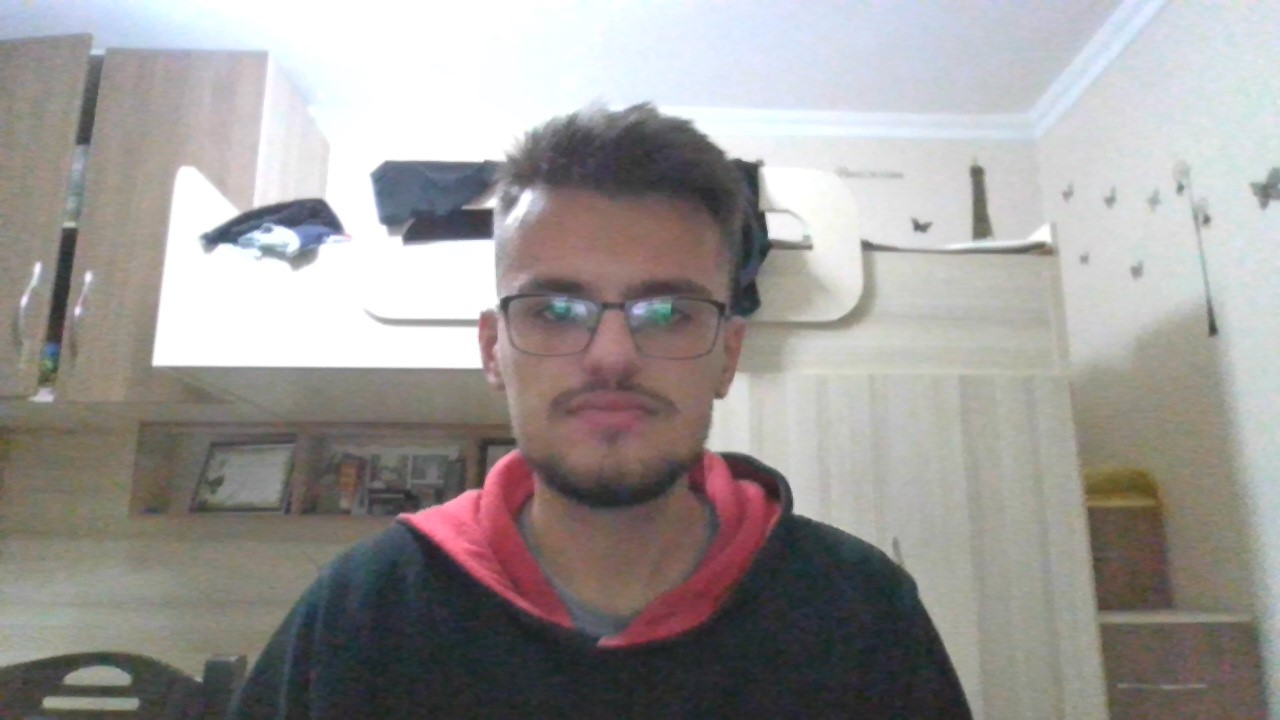
\includegraphics[width=0.9\textwidth]{./figures/jordiR.jpg}
      \caption{Reale Person}
\end{figure}
\begin{figure}[ht]
  \centering
    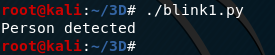
\includegraphics[width=0.9\textwidth]{./figures/detected.png}
      \caption{Ausgabe: Person Detected}
\end{figure}

\newpage
Als zweites Beispiel wird ein Bild von einem Kind genommen, und vor der Kamera gehalten. Dieses Mal ist das Ergebnis anders, das Progamm liefert keine Nachricht zurück. Das Programm läuft weiter bis wirklich eine Person vor der Kamera steht, sonst wartet das System auf eine Rückmeldung.
\begin{figure}[ht]
  \centering
    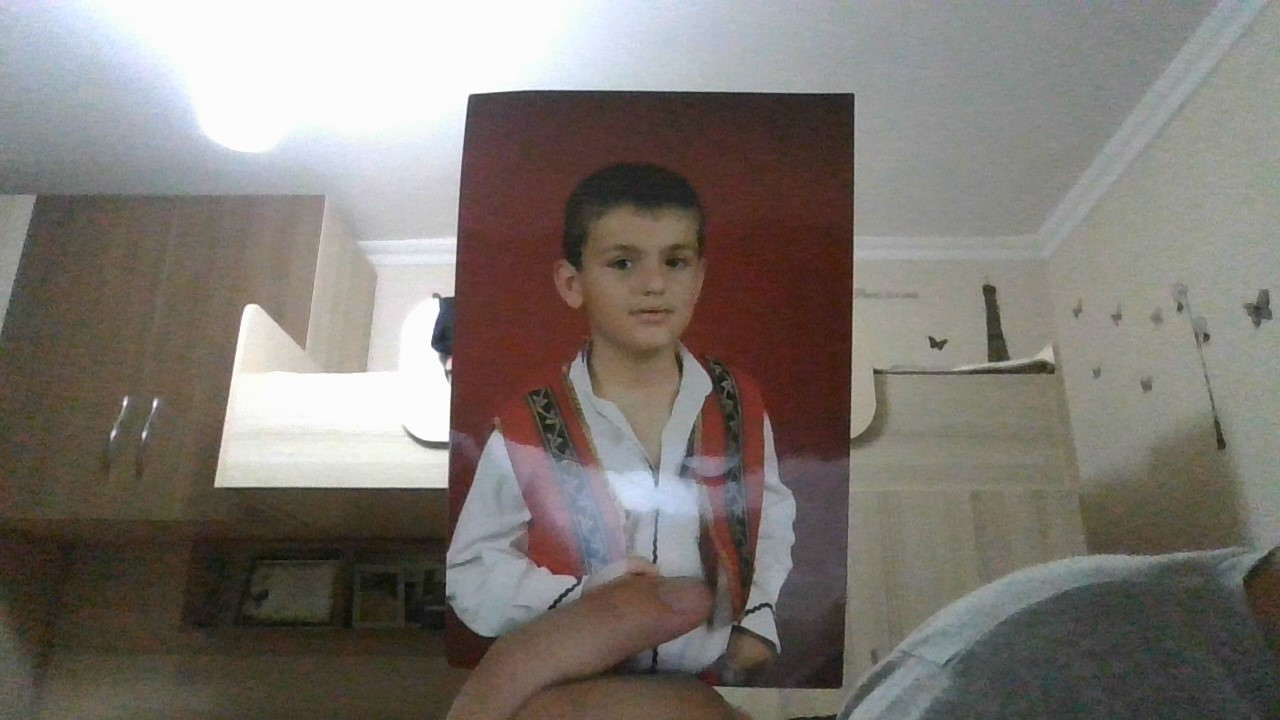
\includegraphics[width=0.9\textwidth]{./figures/kind.jpg}
      \caption{Bild eines Kindes}
\end{figure}
\begin{figure}[ht]
  \centering
    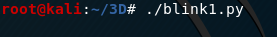
\includegraphics[width=0.9\textwidth]{./figures/ndetected.png}
      \caption{Ausgabe: Nicht Detected}
\end{figure}
\subsubsection{Zeitdauer}
Ziel des Systems ist das Gesicht je schnell wie möglich zu erkennen. Deshalb wurden ein paar Testfällen durchgeführt, in denen die Länge dieses Antispoofing Programms gatestet wurde. Auf den Bildern sind 3 verschiedene Zeitdauern, aber die wichtigste, ist die reale Zeitdauer. Die reale Zeitdauer misst die Zeit, vom Start des Programms bis zum Ende. Im Durschnitt, mit dem Einschalten der Kamera, braucht das Programm ca. 4.4 Sekunden um eine reale Person zu erkennen.
\begin{figure}[!htb]
   \begin{minipage}{0.48\textwidth}
     \centering
     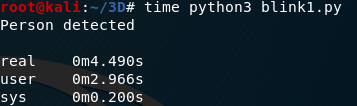
\includegraphics[width=.9\linewidth]{./figures/time1.png}
     \caption{Zeitdauer 1}
   \end{minipage}\hfill
   \begin{minipage}{0.48\textwidth}
     \centering
     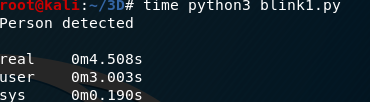
\includegraphics[width=.9\linewidth]{./figures/time2.png}
     \caption{Zeitdauer 2}
   \end{minipage}
\end{figure}
\begin{figure}[!htb]
   \begin{minipage}{0.48\textwidth}
     \centering
     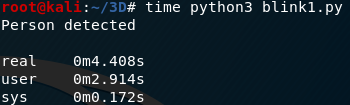
\includegraphics[width=.9\linewidth]{./figures/time3.png}
     \caption{Zeitdauer 3}
   \end{minipage}\hfill
   \begin{minipage}{0.48\textwidth}
     \centering
     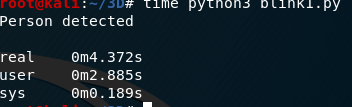
\includegraphics[width=.9\linewidth]{./figures/time4.png}
     \caption{Zeitdauerl 4}
   \end{minipage}
\end{figure}
\newpage
\section{Herausforderungen}
Jedes Projekt hat seine Herausforderungen, und wenn etwas schief geht sollten Alternativen gefunden werden. Auch in diesem Projekt gab es solche Probleme, die durch Hilfe von Tutorials und Blogs gelöst wurden.
\subsection{Datenkbank - MariaDB}
Die meisten Probleme sind bei der Datenbank aufgetreten, wegen der kleinen Unterschiede zwischen MySQL und MariaDB. Manchmal wurde mit dem Progammierregeln von MySQL gearbeitet, obwohl MariaDB in Verwendung war. Zwischen diese zwei Datenbankverwaltungssystem gibt es kleine Unterschiede, die zu Problemen fuhren. Die eingetretenen Fehler werden nun besprochen:
\bigbreak
\textit{ERROR 1452: Cannot add or update a child row: a foreign key constraint fails.}
Das Problem hier war, dass keine Tabelle geändert werden konnte, wegen der Beziehungen zwischen Tabellen. In Prinzip sollte zuerst die Kind Tabelle gelöscht werden, und dann die Eltern Tabelle, weil sonst gibt es eine Konflikt, weil bei der Kind Tabelle einen Fremdschlüssel definiert ist, auf die Tabelle verweisst.
\bigbreak
\begin{figure}[ht]
  \centering
    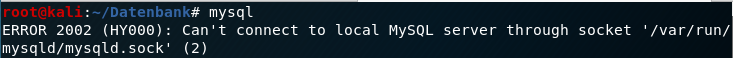
\includegraphics[width=0.9\textwidth]{./figures/fehler1.png}
      \caption{Mysql-Server is missing}
\end{figure}
\textit{You have an error in your SQL syntax; check the manual that corresponds to your mariadb server version for the right syntax to use near .. At line 1}\\
Dieser Fehler wurde ausgelöst, wenn ein Trigger Script ausgeführt wurde. Der Fehler ist beim Delimiter aufgetreten, weil wenn ein Trigger durch ein Script erstellet wird, braucht man keine Delimiter, sondern nur wenn es manuell durch die Command Line ausgeführt wird, musste der Delimiter festgelegt werden. Hier kann man die Unterschied zwischen MariaDB und MySQL sehen, in MySQL wird dieser Code ohne Probleme ausgeführt.
\bigbreak
\textit{Mysql-Server is missing}\\
Dieser Fehler zeigt, dass kein MySQL Server auf dem Betriebssystem installiert ist. Dieses Problem ist eingetreten, wegen Änderungen im Linux System. MySQL Server wurde nicht mehr unterstützt, Betrieb MariaDB, und statt mysql-server zu installieren, sollte mariadb-server durch den Befehl \textit{sudo apt-get install mariadb-server} installiert werden.


\bigbreak
\textit{ERROR 2002 (HY000): Can't connect to local MySQL server through socket \\'/var/run/mysqld/mysqld.sock' (2 "No such file or directory")}\\
Dass war nur ein kleiner Fehler, weil wenn man in Kali Linux programmiert und gearbeitet hat, musste der MariaDB Server immer noch einmal durch den Befehl \\ \textit{service mariadb restart} gestartet werden. Im Debian Betriebssystem, das auf RaspberryPi installiert ist, muss der Server nicht gestartet werden, weil er automatisch in Betrieb ist.

\subsection{Disparity Map}
Am Begin war geplant, als Antispoofing-Methode die 3D Depth Perception zu implementieren. In dieser Methode werden zwei Kameras gebraucht, wo zwei Bilder gemacht werden, ein von jeder Kamera. Dann werden sie verglichen, um eine 3D Objekt zu erstellen. Zuerst wird eine Mischung von beiden Bildern zum Erstellen eine sogenannten Disparty Map gemacht. Eine Disparity Map ist ein schwarz-weiß Bild, das die Tiefe der einzelnen Objektpunkten darstellt.
\begin{figure}[ht]
  \centering
    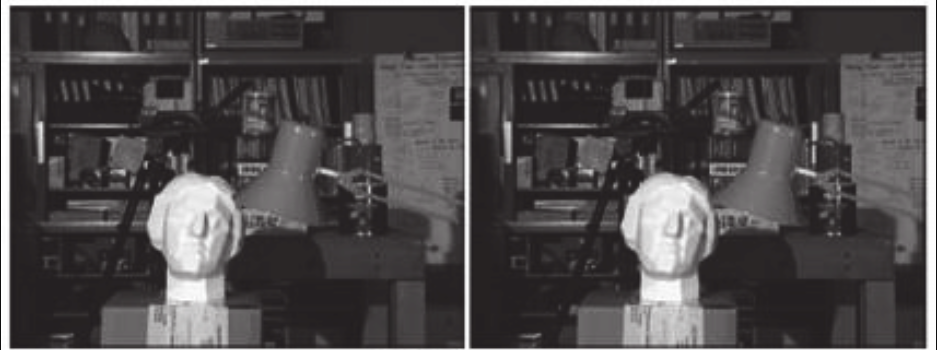
\includegraphics[width=0.9\textwidth]{./figures/disp1.png}
      \caption{Linke und Rechte Bild}
      \cite{disparityM}
\end{figure}
\begin{figure}[ht]
  \centering
    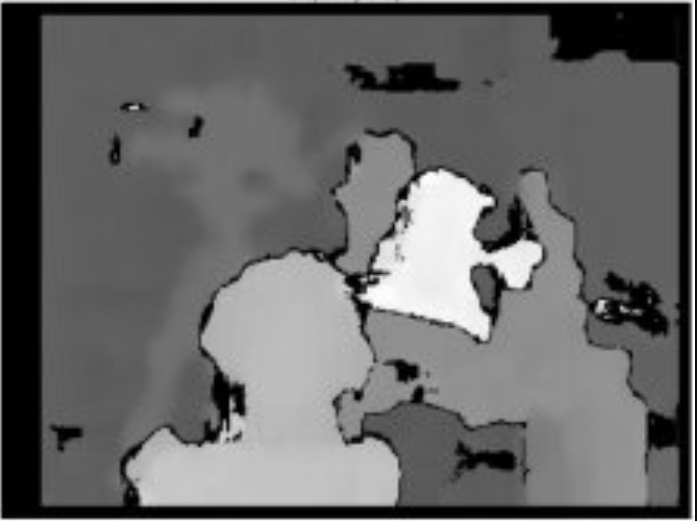
\includegraphics[width=0.5\textwidth]{./figures/disp.png}
      \caption{Beispiel Disparity Map}
      \cite{disparityM}
\end{figure}
\bigbreak
Daher kann die Disparity Map in ein 3D File umgewandelt werden. Es gibt Programmen, wie MatLab, dass eine Matplotlib Bibliothek hat, um dieses Disparity Map in einem 3D Graph zu zeigen. Wenn man die 3D Koordinaten eines Punktes hat, kann man verschiedene Punkten vergleichen z.B Nasen Punkten mit Augen Punkten. So wird gezeigt, dass diese Punkten verschiedene Distanzen von der Kamera haben. Während ein normales Bild als 2D dargestellt wird, und so kennt das Programm automatisch, dass vor der Kamera ein Bild und nicht eine reale Person ist.
\begin{figure}[ht]
  \centering
    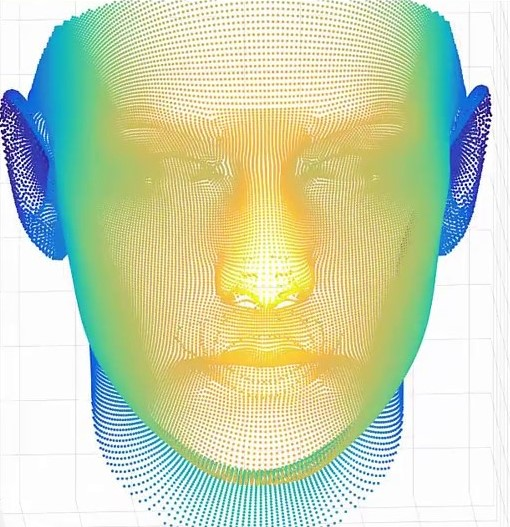
\includegraphics[width=0.7\textwidth]{./figures/matlib.jpg}
      \caption{3D Gesicht Matlab}
      \cite{matlab}
\end{figure}
\bigbreak
Die große Herausforderung war die Recherche und Erstellen von Disparity Map. Das Tutorial bzw. die Dokumentation waren entweder waren sehr kurz erklärt und veraltet, oder sehr anspruchsvoll. Nach ein paar Tests vom Erstellen von Disparity Maps war die Erfolgsrate gering, eine von drei Disparity Maps wurde  richtig erzeugt.
\bigbreak
\newpage
Aus dem ersten Beispiel wurde eine gute Disparity Map erzeugt, und mit dieser Disparity Map kann man bis zur 3D Umwandlung  weiterarbeiten.
\begin{figure}[!htb]
   \begin{minipage}{0.48\textwidth}
     \centering
     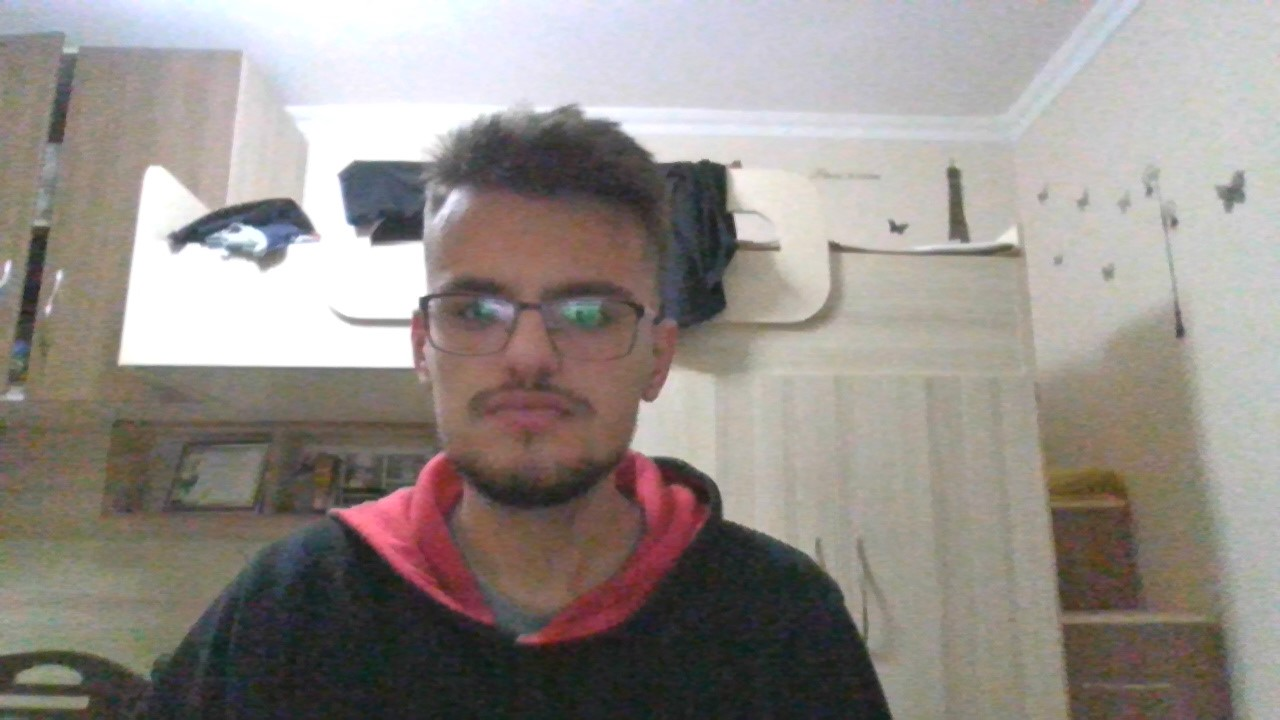
\includegraphics[width=.9\linewidth]{./figures/jordiL.jpg}
     \caption{Jordi Linke Bild 1}
   \end{minipage}\hfill
   \begin{minipage}{0.48\textwidth}
     \centering
     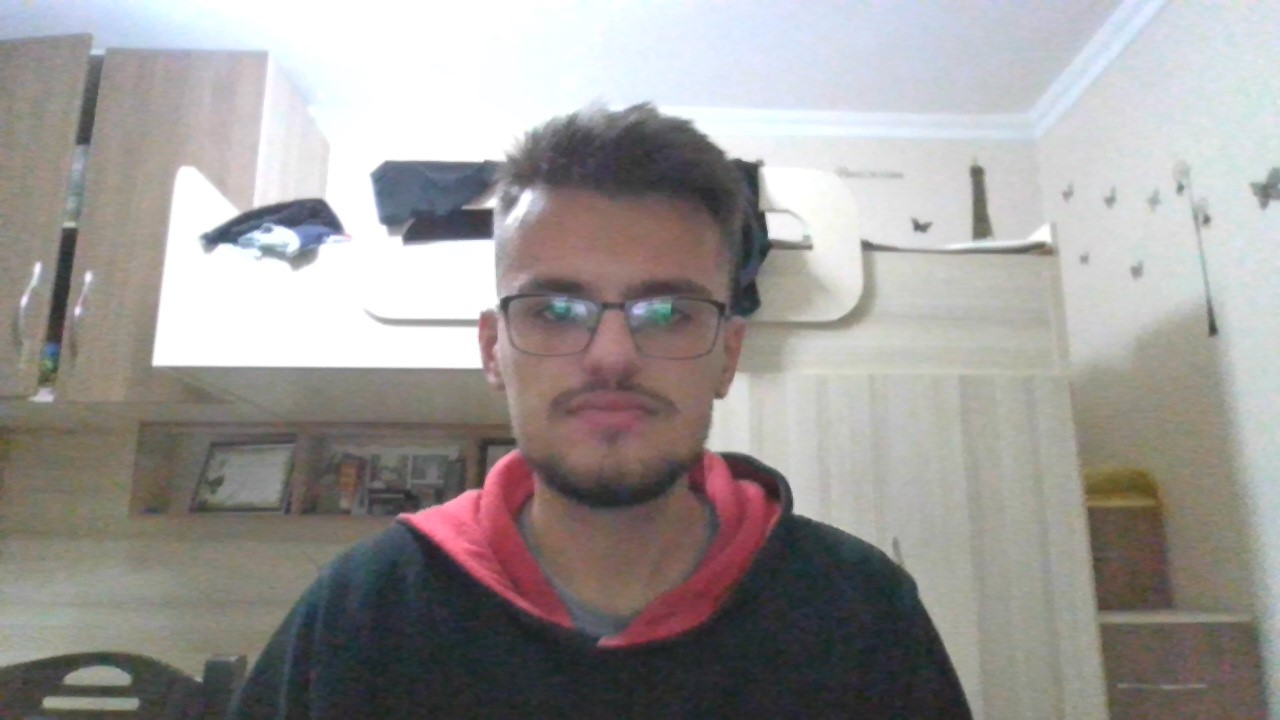
\includegraphics[width=.9\linewidth]{./figures/jordiR.jpg}
     \caption{Jordi Linke Bild 1}
   \end{minipage}
\end{figure}
\begin{figure}[!htb]
  \centering
    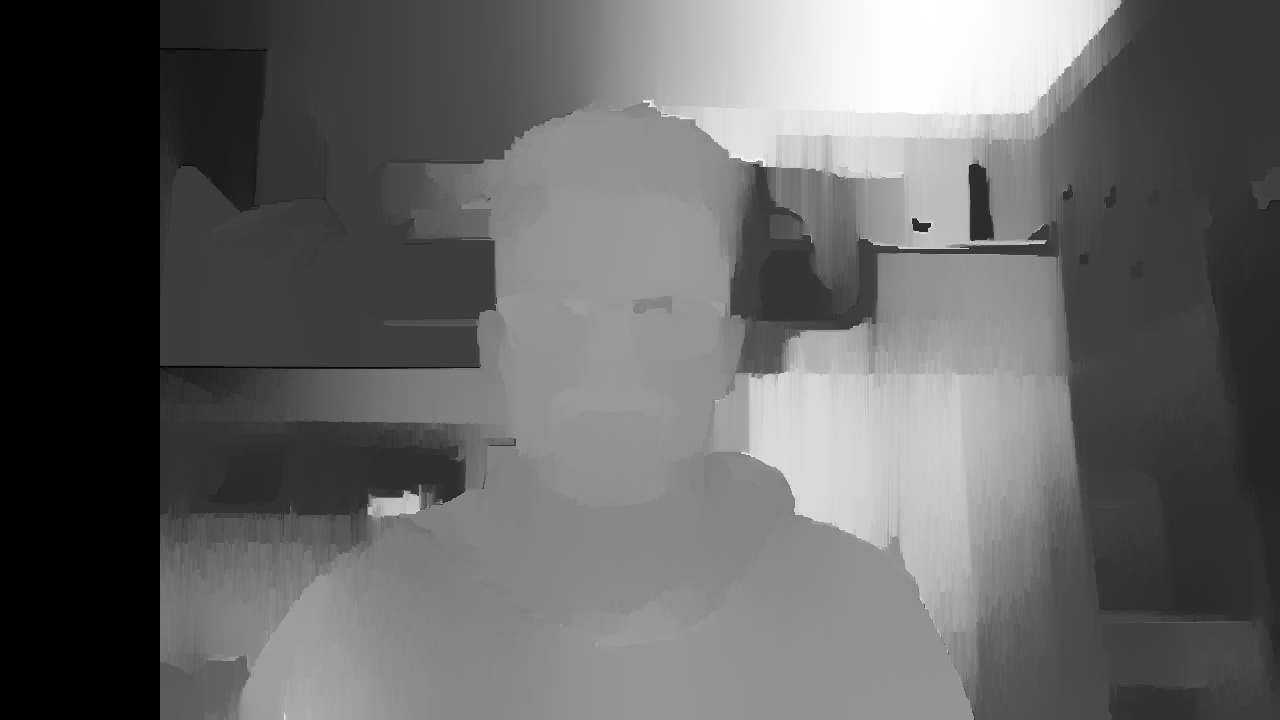
\includegraphics[width=0.9\textwidth]{./figures/dispgood.jpg}
      \caption{Gutes Disparity Map}
\end{figure}\\
Aber aus den anderen Bildern wurde keine gute Disparity Map erzeugt. Mit dieser Disparity Map war die 3D Umwandlung nicht realisierbar.
\begin{figure}[!htb]
   \begin{minipage}{0.48\textwidth}
     \centering
     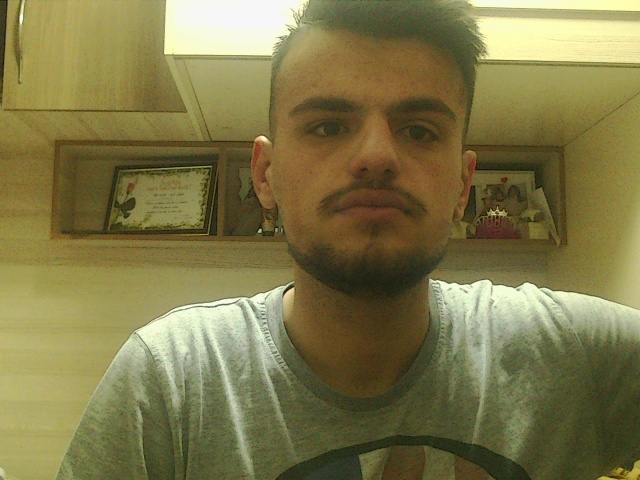
\includegraphics[width=.7\linewidth]{./figures/frameL.jpg}
     \caption{Jordi Linke Bild 2}
   \end{minipage}\hfill
   \begin{minipage}{0.48\textwidth}
     \centering
     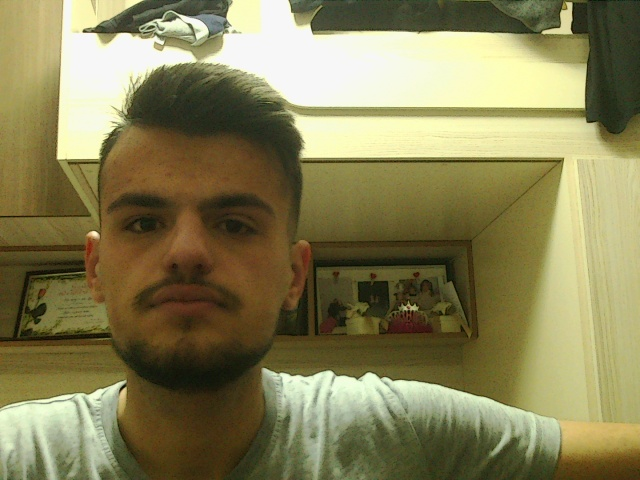
\includegraphics[width=.7\linewidth]{./figures/frameR.jpg}
     \caption{Jordi Linke Bild 2}
   \end{minipage}
\end{figure}
\begin{figure}[!htb]
  \centering
    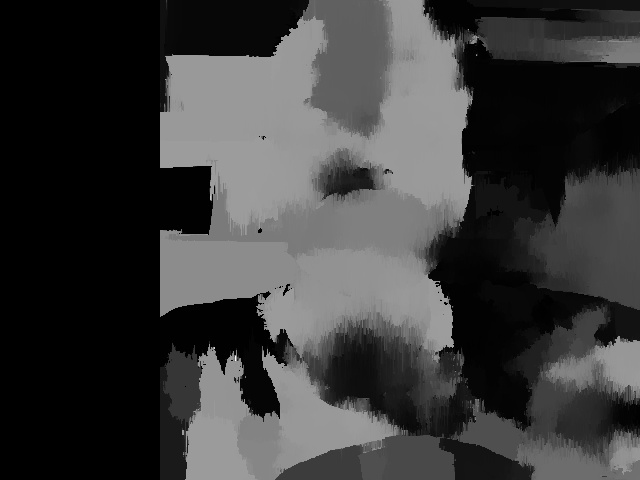
\includegraphics[width=0.7\textwidth]{./figures/dispbad.jpg}
      \caption{Schlechtes Disparity Map}
\end{figure}
\newpage
\subsection{Python Scripting}
Python ist eine beliebte Programmiersprachen von vielen Benutzern, aber Python unterscheidet sich von anderen Programmiersprachen durch die Code Struktur. Die meisten Fehler wurden bei der Übertragung von den Parametern zwischen den verschieden Funktionen erzeugt.
\bigbreak
\textit{TypeError: not all arguments converted during string formatting python}\\
Der folgende Code nimmt als Parameter die Daten von dem neuen User, damit der User in der Datenbank registriert wird. Aber wenn man die Methode nur testen möchte, und als Parameter nur der Name für eine einfache Registrierung übergibt, dann tritt dieser Fehler ein. \\\\
\textit{insertvalues1(curs,'jordi','zmiani','jorzmi14@htl-shkoder.com',1)}\\\\
Bei der ersten Möglichkeit sollten zwei Parameter übergeben werden, denn nur bei einem String Parameter wurde dieser Fehler generiert.
Bein der zweiten Möglichkeit musst dieser Parameter durch die Funktion format()  geparst werden.
\bigbreak
\textit{TypeError: 'str' object is not callable (Python)}\\
Str in Python ist eine spezielle Methode, und diese Methode sollte nicht überschrieben werden, das heißt, dass es keine Variable bzw. Funktion mit diesem Namen erstellet werden  sollte. Aber trotzdem wurde dieser Fehler generiert, weil er auftritt, wenn ein Parameter auf den falschen Datentyp geparst wird.

\subsection{OpenCV}
OpenCV Biblotheken können manchmal schwierig zu installieren sein, weil es so viele Möglichkeiten zum Einrichten von OpenCV gibt, die aber von dem Betriebsystem abhängen. In den meisten Fällen, wenn die Installation Fehler produziert, muss OpenCV, noch einmal von Beginn eingerichtet werden.
\bigbreak
\textit{Unable to locate package libjasper-dev}\\
Diese Package ermöglicht ein paar Funktion von den OpenCV, das ist eine von vielen Bibliotheken, die eingebunden werden soll. In diesem Fall konnte diese Bibliothek nicht installiert werden, weil sich die Repository geändert haben, und deshalb mussten die Bibliotheken in einer älteren Version heruntergeladen werden. Mit den folgenden Befehlen wurden diese Bibliotheken installiert.\\\\
\textit{echo "deb http://us.archive.ubuntu.com/ubuntu/ yakkety universe" | sudo tee -a \\ /etc/apt/sources.list}\\
\textit{sudo apt update}\\
\textit{sudo apt install libjasper1 libjasper-dev}

\section{Qualitätssicherung}
\textit{"Einer der wohl bekanntesten Berater, Lehrer und Autoren zum Thema Qualität ist der Amerikaner W. Edwards Deming. Deming
entwickelte auf der Basis der allgemeinen Problemlösungsmethode den sogenannten Plan-Do-CheckAct-Zyklus (PDCA-Zyklus). Auf der Plan-Phase werden Probleme betrachtet und Lösungsmaßnahmen
erarbeitet. Die Do-Phase ist die Phase der Umsetzung bzw. Ausführung der zuvor gefundenen
Lösungen. In der Check-Phase wird bewertet, ob die Maßnahmen zum Erfolg geführt haben.
Innerhalb der nachfolgenden Act-Phase findet eine Standardisierung der erfolgreichen Maßnahmen
statt, die fortan als Basis für weitere Verbesserungen dient."}\cite{PDCA-Zyklus}
\bigbreak 
\begin{figure}[!htb]
  \centering
    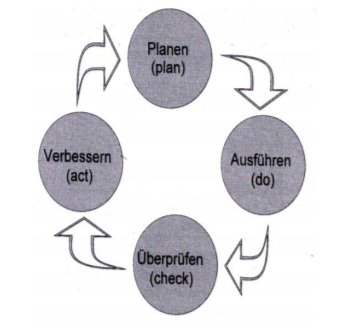
\includegraphics[width=0.7\textwidth]{./figures/pdca.png}
      \caption{Plan-Do-Check-Act-Zyklus}
    \label{fig:pdca}
	\cite{PDCA-Zyklus}
\end{figure}
Auf dem Bild \ref{fig:pdca} wird der PDCA Zyklus dargestellte. Man sieht, dass diese Qualitätsmethode gut für die Verbesserung von Software und Programmen geeignet ist. Deshalb wurde auch diese Methode gewählt, weil durch Error Checking konnten die Fehler gefunden, analysiert und verbessert werden. Das passt gut zum Team, da es keine Erfahrungen mit bestimmenden Programmiersprachen bzw. Softwareprogrammen gab.
\bigbreak
Bei den Herausforderungen (Kapitel 3.3) war klar, dass wenn Probleme erkannt wurden, diese durch Hilfe von Tutorials bzw. Net Blogs gelöst werden. Durch verschiedene Zyklen wird man, wenn etwas nicht funktionier,das Problem  schnell gefunden und später wird ein neuer Lösungsweg bestimmt. So werden die Risiken so früh wie möglich eliminiert.

\newpage
\section{Ergebnisse}
\subsection{Datenbank}
Für den Bereich Datenbank wurde jede Woche programmiert, seit dem Beginn des Projekts wurden Recherchen über verschiedenen Arten von Gesichtserkennungs der Datenbanken gemacht, und später hat die Planung und das Design der Datenbank begonnen. Es gab viele Änderungen abhängig von den anderen Teilbereichen des Projektes. Die Datenbank musste immer geändert werden, und an die Gesichtsdaten angepasst werden. Die folgenden Punkten der Datenbank wurden realisiert:
\begin{itemize}
	\item Datenbankdesign
	\item Erstellen von Tabellen
	\item Triggers \& Proceduren
	\item Zugriffsrechte
	\item Datenbank Backup
\end{itemize}
\subsection{2D vs. 3D Unterschied}
In diesem Bereich gab es viele Herausforderungen und Änderungen, deshalb ist der Lösungsweg mehrmals geändert oder aktualisiert werden. Zu Beginn war geplant, mit Hilfe von zwei Kameras die Tiefe des Bildes zu finden, und danach mit dieser Tiefe weiterzuarbeiten. Aber dass war schwierig umsetzbar, daher wurde ein anderer Lösungsweg gefunden. Nun wird eine Person mit Hilfe von  Blinzeln identifiziert.

